\chapter{Enzymes}\label{enzymes}

\href{https://en.wikipedia.org/wiki/Enzyme}{Enzymes} are macromolecular
biological catalysts. The molecules upon which enzymes may act are
called substrates and the enzyme converts the substrates into different
molecules known as products. Almost all metabolic processes in the cell
need enzyme catalysis in order to occur at rates fast enough to sustain
life. Metabolic pathways depend upon enzymes to catalyze individual
steps. Enzymes are known to catalyze more than 5,000 biochemical
reaction types. Most enzymes are proteins, although a few are catalytic
RNA molecules. The latter are called ribozymes. Enzymes' specificity
comes from their unique three-dimensional structures.

Like all catalysts, enzymes increase the reaction rate by lowering its
activation energy. Some enzymes can make their conversion of substrate
to product occur many millions of times faster. An extreme example is
orotidine 5'-phosphate decarboxylase, which allows a reaction that would
otherwise take millions of years to occur in milliseconds. Chemically,
enzymes are like any catalyst and are not consumed in chemical
reactions, nor do they alter the equilibrium of a reaction. Enzymes
differ from most other catalysts by being much more specific. Enzyme
activity can be affected by other molecules: inhibitors are molecules
that decrease enzyme activity, and activators are molecules that
increase activity. Many therapeutic drugs and poisons are enzyme
inhibitors. An enzyme's activity decreases markedly outside its optimal
temperature and pH.

Some enzymes are used commercially, for example, in the synthesis of
antibiotics. Some household products use enzymes to speed up chemical
reactions: enzymes in biological washing powders break down protein,
starch or fat stains on clothes, and enzymes in meat tenderizer break
down proteins into smaller molecules, making the meat easier to chew.

In this laboratory, we will study the effect of temperature,
concentration and pH and on the activity of the enzyme catalase.
Catalase speeds up the following reaction:

2 H\textsubscript{2}O\textsubscript{2} -\textgreater{} 2
H\textsubscript{2}O + O\textsubscript{2}

Hydrogen peroxide is toxic cells protect themselves. Cells therefore use
catalase to protect themselves. In these experiments, we will use
catalase enzyme from potato.

The first experiment will establish that our catalase works (positive
control) and that our reagents are not contaminated (negative control).

Hydrogen peroxide will not spontaneously degrade at room temperature in
the absence of enzyme. When catalase is added to hydrogen peroxide, the
reaction will take place and the oxygen produced will lead to the
formation of bubbles in the solution. The height of the bubbles above
the solution will be our measure of enzyme activity (Figure
\ref{fig:catalase}).

\begin{figure}

{\centering 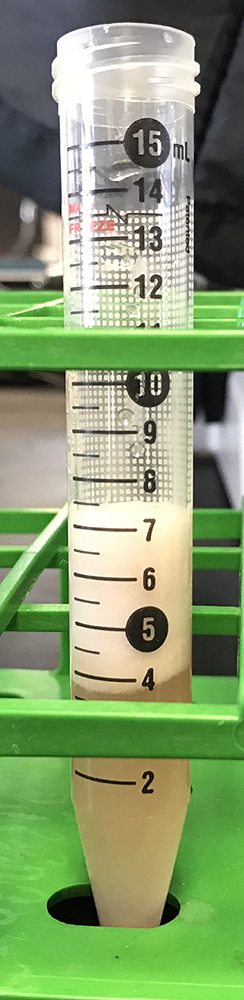
\includegraphics[width=0.7\linewidth]{./figures/enzymes/catalase}

}

\caption{Catalase in action. Note the white bubbles above the darker liquid.}\label{fig:catalase}
\end{figure}

\section{Positive and negative controls (Experiment
1)}\label{positive-and-negative-controls-experiment-1}

\subsection{Experimental procedures}\label{experimental-procedures-17}

\begin{enumerate}
\def\labelenumi{\arabic{enumi}.}
\tightlist
\item
  Obtain and label three tubes.
\item
  Then to \textbf{Tube 1}

  \begin{itemize}
  \tightlist
  \item
    Add 1 ml of potato juice (catalase) to tube 1 (use a plastic
    transfer pipette).
  \item
    Add 4 ml of hydrogen peroxide to tube 1. Swirl well to mix and wait
    at least 20 seconds for bubbling to develop.
  \item
    Use a ruler and measure the height of the bubble column above the
    liquid (in millimeters; use the centimeter scale of the ruler) and
    record the result in Table \ref{tab:control}.
  \end{itemize}
\item
  Then to \textbf{Tube 2}

  \begin{itemize}
  \tightlist
  \item
    Add 1 ml of water.
  \item
    Add 4 ml of hydrogen peroxide. Swirl well to mix and wait at least
    20 seconds.
  \item
    Measure the height of the bubble column (in millimeters) and record
    the result in Table \ref{tab:control}.
  \end{itemize}
\item
  Then to \textbf{Tube 3}

  \begin{itemize}
  \tightlist
  \item
    Add 1 ml of potato juice (catalase).
  \item
    Add 4 ml of sucrose solution. Swirl well to mix; wait 20 seconds.
  \item
    Measure the height of the bubble column and record the result in
    Table \ref{tab:control}.
  \end{itemize}
\end{enumerate}

\begin{longtable}[]{@{}cl@{}}
\caption{\label{tab:control} Positive and negative controls.}\tabularnewline
\toprule
Tube \# & Height of bubbles (mm)\tabularnewline
\midrule
\endfirsthead
\toprule
Tube \# & Height of bubbles (mm)\tabularnewline
\midrule
\endhead
1 &\tabularnewline
2 &\tabularnewline
3 &\tabularnewline
\bottomrule
\end{longtable}

\section{Effect of temperature on enzyme activity (Experiment
2)}\label{effect-of-temperature-on-enzyme-activity-experiment-2}

\subsection{Experimental procedures}\label{experimental-procedures-18}

\begin{enumerate}
\def\labelenumi{\arabic{enumi}.}
\tightlist
\item
  Obtain and label three tubes.
\item
  Add 1 ml of potato juice (catalase) to each tube.
\item
  Place tube 1 in the refrigerator, tube 2 in a 37°C (Celsius) heat
  block, and tube 3 in a 97°C heat block for 15 minutes.
\item
  Remove the tubes with the potato juice (catalase) from the
  refrigerator and heat blocks and immediately add 4 ml hydrogen
  peroxide to each tube.
\item
  Swirl well to mix and wait 20 seconds.
\item
  Measure the height of the bubble column (in millimeters) in each tube
  and record your observations in Table \ref{tab:temp}.
\end{enumerate}

\begin{longtable}[]{@{}cl@{}}
\caption{\label{tab:temp} Effect of temperature on enzyme
activity.}\tabularnewline
\toprule
Tube \# & Height of bubbles (mm)\tabularnewline
\midrule
\endfirsthead
\toprule
Tube \# & Height of bubbles (mm)\tabularnewline
\midrule
\endhead
1 &\tabularnewline
2 &\tabularnewline
3 &\tabularnewline
\bottomrule
\end{longtable}

\section{Effect of concentration on enzyme activity (Experiment
3)}\label{effect-of-concentration-on-enzyme-activity-experiment-3}

\subsection{Experimental procedures}\label{experimental-procedures-19}

\begin{enumerate}
\def\labelenumi{\arabic{enumi}.}
\tightlist
\item
  Obtain and label three tubes.
\item
  Then to \textbf{Tube 1}

  \begin{itemize}
  \tightlist
  \item
    Add 1 ml of water.
  \item
    Add 4 ml of hydrogen peroxide. Swirl well to mix and wait at least
    20 seconds.
  \item
    Measure the height of the bubble column (in millimeters) and record
    your observations in Table \ref{tab:concentration}.
  \end{itemize}
\item
  Then to \textbf{Tube 2}

  \begin{itemize}
  \tightlist
  \item
    Add 1 ml of potato juice (catalase).
  \item
    Add 4 ml of hydrogen peroxide. Swirl well to mix and wait at least
    20 seconds.
  \item
    Measure the height of the bubble column (in millimeters) and record
    your observations in Table \ref{tab:concentration}.
  \end{itemize}
\item
  Then to \textbf{Tube 3}

  \begin{itemize}
  \tightlist
  \item
    Add 3 ml of potato juice (catalase).
  \item
    Add 4 ml of hydrogen peroxide. Swirl well to mix and wait at least
    20 seconds.
  \item
    Measure the height of the bubble column (in millimeters) and record
    your observations in Table \ref{tab:concentration}.
  \end{itemize}
\end{enumerate}

\begin{longtable}[]{@{}cl@{}}
\caption{\label{tab:concentration} Effect of concentration on enzyme
activity.}\tabularnewline
\toprule
Tube \# & Height of bubbles (mm)\tabularnewline
\midrule
\endfirsthead
\toprule
Tube \# & Height of bubbles (mm)\tabularnewline
\midrule
\endhead
1 &\tabularnewline
2 &\tabularnewline
3 &\tabularnewline
\bottomrule
\end{longtable}

\section{Effect of pH on enzyme activity (Experiment
4)}\label{effect-of-ph-on-enzyme-activity-experiment-4}

\subsection{Experimental procedures}\label{experimental-procedures-20}

\begin{enumerate}
\def\labelenumi{\arabic{enumi}.}
\tightlist
\item
  Obtain 6 tubes and label each tube with a number from 1 to 6.
\item
  Place the tubes from left (tube \#1) to right (tube \#6) in the first
  row of a test tube rack.
\item
  Add to 1 ml of potato juice (catalase) to each tube.
\item
  Add 2 ml of water to tube 1.
\item
  Add 2 ml of pH buffer 3 to tube 2.
\item
  Add 2 ml of pH buffer 5 to tube 3.
\item
  Add 2 ml of pH buffer 7 to tube 4.
\item
  Add 2 ml of pH buffer 9 to tube 5.
\item
  Add 2 ml of pH buffer 12 to tube 6.
\item
  Add 4 ml of hydrogen peroxide to each of the six tubes.
\item
  Swirl each tube well to mix and wait at least 20 seconds.
\item
  Measure the height of the bubble column (in millimeters) in each tube
  and record your observations in Table \ref{tab:pH}.
\end{enumerate}

\begin{longtable}[]{@{}cl@{}}
\caption{\label{tab:pH} Effect of pH on enzyme activity.}\tabularnewline
\toprule
Tube \# & Height of bubbles (mm)\tabularnewline
\midrule
\endfirsthead
\toprule
Tube \# & Height of bubbles (mm)\tabularnewline
\midrule
\endhead
1 &\tabularnewline
2 &\tabularnewline
3 &\tabularnewline
4 &\tabularnewline
5 &\tabularnewline
6 &\tabularnewline
\bottomrule
\end{longtable}

\section{Cleaning up}\label{cleaning-up-5}

\begin{enumerate}
\def\labelenumi{\arabic{enumi}.}
\tightlist
\item
  Empty the contents of the plastic tubes into the labeled waste
  container (brown bottle) in the chemical fume hood.
\item
  Discard the empty tubes and other waste in the regular waste basket.
\item
  Rinse the glass rod and glassware with water and detergent.
\item
  Return the glass ware to the trays on your bench where you originally
  found them.
\end{enumerate}

\section{Review Questions}\label{review-questions-4}

\begin{enumerate}
\def\labelenumi{\arabic{enumi}.}
\tightlist
\item
  What is a catalyst?
\item
  What are enzymes?
\item
  What is the name of the enzyme that we studied in this laboratrory
  session?
\item
  What is an enzyme substrate?
\item
  What is the substrate of the enzyme that we used in this laborator
  seesion?
\item
  What are the products of the reachtion that was catalized by the
  enzyme that we studied in this laboratory seesion?
\item
  What is the active site of an enzyme?
\item
  What is the purpose of the negative and positive controls?
\item
  State the hypothesis that was tested in experiment 2?
\item
  State the hypothesis that was tested in experiment 3?
\item
  State the hypothesis that was tested in experiment 4?
\item
  The enzyme from potato appeared to work better at 4°C than at 37°C.
  Would you expect the same if we had used the equivalent human enzyme?
  Justify your answer.
\item
  Why did heating the enzyme at high heat (\textgreater{} 65°C) result
  in loss of activity?
\end{enumerate}
